\section{Introduction to Mathematical Framework}

This work develops a concise mathematical framework for how higher–dimensional vortex structures manifest in three spatial dimensions. The central object is a codimension–2 vortex sheet $\Sigma\subset\mathbb{R}^4$ with sheet strength $\Gamma$, observed on a three–dimensional slice $\Pi=\{w=0\}$. Our aims are to keep assumptions explicit, maintain dimensional consistency, and produce testable statements with controlled error estimates.

\paragraph{Roadmap in pictures.}
The framework builds around six core physical concepts, each with a concrete analogy:
\begin{itemize}
  \item \textbf{Intake}: Like water flowing down a sink drain--gentle, universal inflow
  \item \textbf{Slope}: Like a standing hill or valley--the electric potential landscape
  \item \textbf{Eddies}: Like whirlpools in a stream--closed circulation patterns ($\mathbf{B}$ field)
  \item \textbf{Twist}: Like a torsion spring--hidden cross-slab circulation maintaining the vortex
  \item \textbf{Induction}: Like a transformer ring--electric loops when magnetic eddies change
  \item \textbf{Drag}: Like sideways pull through honey--organizes eddies when cores move
\end{itemize}
These concepts map directly to observable fields: Intake $\to$ gravity, Slope+Induction $\to$ $\mathbf{E}$ field, Eddies $\to$ $\mathbf{B}$ field, with Twist providing maintenance and Drag organizing motion.

\paragraph{Scope.}
The framework provides:
(i) a representation of vortex sheets in $\mathbb{R}^4$ suitable for projection,
(ii) a map from 4D structure to 3D observables on $\Pi$,
(iii) a decomposition of slice fields into divergence–free (circulatory) and gradient (potential or ``drainage'') parts, and
(iv) scaling relations with explicit error control in the thin/flat limit.
Small parameters are the core–to–loop aspect ratio $\xi/\rho$ and the slice–scale curvature $\kappa\rho$, with typical remainder terms $O\!\left((\xi/\rho)^2+(\kappa\rho)^2\right)$.

\paragraph{Projection principle.}
When a small loop $\gamma\subset\Pi$ links the projected intersection $\Sigma\cap\Pi$ once, the circulation measured on the slice equals the sheet strength:
\[
\oint_{\gamma} \mathbf{v}\cdot d\boldsymbol{\ell}\;=\;\Gamma
\quad\text{(thin/flat limit),}
\]
with the total arising from two equal \emph{half–space} contributions across the slice, each $\Gamma/2$. Potential (drainage) adjustments on the slice are gradient fields and contribute zero to the loop integral. \textit{If you only remember one thing:} Circulation projects; drainage doesn't.

\paragraph{Kernel normalization (summary).}
Where an explicit kernel is required, we use the correctly normalized 4D$\to$3D Biot–Savart–type expression for an axially symmetric configuration, yielding the standard azimuthal profile
\[
v_\theta(\rho)
=\frac{\Gamma}{4\pi\rho}\!\int_{-\infty}^{\infty}\frac{\rho^2\,dw}{(\rho^2+w^2)^{3/2}}
=\frac{\Gamma}{2\pi\rho}.
\]
The one–sided integrals over $w>0$ and $w<0$ each produce $\Gamma/2$, making the half–space split explicit and consistent with the projection principle above.

\begin{physbox}[title=Orientation note]
We take $\Gamma>0$ to correspond to circulation given by the right–hand rule around the oriented sheet normal. This fixes the sign in the azimuthal profile.
\end{physbox}

\paragraph{Decomposition on the slice.}
Fields on $\Pi$ are organized into a solenoidal component that carries the circulation and a curl–free potential component determined by continuity. Only the solenoidal part contributes to loop integrals; the potential part can influence local velocities and pressures but integrates to zero circulation around closed loops.

\paragraph{Outline and related results.}
Subsequent sections apply the projection principle and kernel identities to derive practical expressions for observables on $\Pi$, quantify finite–core and curvature corrections, and state verification procedures amenable to numerical checks. For hierarchical vortex energetics that lead to the appearance of the golden ratio, a full derivation is provided externally in Norris (2025) \cite{Norris2025GoldenRatio}; this manuscript references that result where relevant without reproducing its proof.

\begin{tcolorbox}[title=Terminology spine (plain language)]
\textbf{Intake} (gravity-like): gentle, charge-blind inflow every core has.
\textbf{Slope} (Coulomb piece of $\,\mathbf E$): the standing hill/valley pattern written by an oriented link.
\textbf{Eddies} (the $\mathbf B$ field): the on-slice circulation map (whirls with no loose ends), organized by motion/drag.
\textbf{Twist} (hidden maintenance): a tiny cross-slab circulation at the core that keeps the rim open; gives a weak $1/r^3$ dipole at rest.
\textbf{Induction} (loop $\,\mathbf E$): the ring-shaped push that appears when eddies change in time.
\textbf{Drag} (organizer of $\mathbf B$): the sideways tug a moving core exerts on the medium; it organizes on-slice Eddies.
\end{tcolorbox}

\paragraph{Electromagnetism (pointer).}
The full EM projection, field definitions, Maxwell dynamics, covariant packaging, wave equations with retarded solutions, and experimental bounds are presented in Sec.~\ref{sec:EM_projection}.

\emph{Note:} Intake, Slope, Eddies, and Twist are the core four; Drag organizes Eddies, and Induction is the loop-$\mathbf E$ that appears when Eddies change in time.

\begin{tcolorbox}[colback=gray!5,colframe=gray!35!black,arc=1mm,boxrule=0.3pt,left=1mm,right=1mm,top=0.5mm,bottom=0.5mm]
\textbf{Do-not-confuse:}
\begin{itemize}
  \item Twist (hidden, maintenance) $\neq$ Eddies (visible $\mathbf B$)
  \item Slope (Coulomb) $\neq$ Induction (loop $\mathbf E$)
  \item Intake (gravity) $\neq$ Drag (organizer of $\mathbf B$)
\end{itemize}
\end{tcolorbox}

\subsection{Foundational Postulates}
\label{sec:foundational-postulates}

We model a codimension–2 vortex sheet $\Sigma\subset\mathbb{R}^4$ intersected by an observed three–dimensional slice $\Pi\subset\mathbb{R}^4$ (the “lab space”). The sheet carries a constant circulation strength $\Gamma$ with units of circulation,
\[
[\Gamma]=L^2/T,
\]
and the slice inherits the usual Helmholtz (irrotational/solenoidal) decomposition of observable fields.

\paragraph*{Small-parameter bookkeeping.}
Throughout P-1–P-6 we work in the thin/flat regime with
\[
\varepsilon_\xi := \frac{\xi}{\rho}\ll 1,\qquad
\varepsilon_\kappa := \kappa\,\rho \ll 1,
\]
and, unless otherwise noted, we retain terms through first order in $(\varepsilon_\xi,\varepsilon_\kappa)$ and neglect $O(\varepsilon_\xi^2+\varepsilon_\kappa^2)$.

\paragraph*{Orientation and sign convention.}
The sheet $\Sigma$ is oriented, the slice $\Pi$ is oriented, and “positive linking'' is defined by the right–hand rule: the orientation induced on a small loop in $\Pi$ by the oriented normal of $\Sigma$ is taken as the positive sense. Equivalently, Stokes' theorem on $\Pi$ fixes the sign so that positive linking yields positive circulation.

\paragraph{P-1: Geometry and regularity}
\label{post:P1}
The sheet $\Sigma$ is an oriented $C^2$ two–dimensional surface with bounded curvature; near each intersection with $\Pi$ we choose a local tubular neighborhood and coordinates so that $\xi>0$ is a (fixed) microscopic core/healing length and $\kappa$ is the local (slice–scale) curvature. On balls $B_\rho\subset\Pi$ of radius $\rho$, we assume the \emph{thin/flat} regime
\[
0<\xi \ll \rho, \qquad \kappa\rho \ll 1,
\]
so that local coordinates may be chosen in which $\Sigma$ is well approximated by a flat sheet over $B_\rho$, with geometric errors controlled by $O(\varepsilon_\xi^2+\varepsilon_\kappa^2)$.

\begin{physbox}\textbf{Physical picture:} Think: compressible superfluid; defects = holes where phase winds.\end{physbox}

\paragraph{P-2: Sheet strength and circulation}
\label{post:P2}
The sheet carries a constant strength $\Gamma$ (with $[\Gamma]=L^2/T$). The induced tangential velocity on $\Pi$ is solenoidal at leading order, and the circulation around any small loop $\gamma\subset\Pi$ that links $\Sigma$ once (positively) is
\[
\oint_{\gamma}\mathbf{v}\cdot d\boldsymbol{\ell}\;=\;\Gamma.
\]
\emph{Parenthetical conservation note.} This postulate specifies the localized circulation budget at the sheet; global 3D mass/charge continuity is ensured by the 4D description (flux through the $w$–direction acts as the reservoir), so nothing here implies a violation of 3D conservation after projection; see the discussion of continuity in Subsection~\ref{sec:motivation-conventions}.

\begin{physbox}\textbf{Physical picture:} Cores behave like tiny drains into ±w; no depletion on the slice.\end{physbox}

\paragraph{P-3: Slice observables and field decomposition}
\label{post:P3}
Observable fields on $\Pi$ are defined by restriction/projection of the 4D fields to the slice, and admit the Helmholtz decomposition
\[
\mathbf{v}=\mathbf{v}_{\mathrm{irrot}}+\mathbf{v}_{\mathrm{sol}},\qquad
\nabla\times \mathbf{v}_{\mathrm{irrot}}=0,\quad
\nabla\cdot \mathbf{v}_{\mathrm{sol}}=0.
\]
Only $\mathbf{v}_{\mathrm{sol}}$ contributes to loop circulation on $\Pi$ at leading order; $\mathbf{v}_{\mathrm{irrot}}$ contributes to potential (gradient) effects but integrates to zero around closed curves contained in $\Pi$.

\begin{physbox}\textbf{Physical picture:} Bulk re-equilibrates quietly; surface (slice) waves are the photons.\end{physbox}

\paragraph{P-4: Kernel normalization (local axisymmetric model)}
\label{post:P4}
In the local \emph{thin/flat} model, the azimuthal velocity profile around a straight segment of $\Sigma$ piercing $\Pi$ is fixed by kernel normalization. With cylindrical coordinates $(\rho,\theta,w)$ adapted to $\Pi$ and the transverse coordinate $w$, the slice azimuthal velocity satisfies
\[
v_\theta(\rho)
=\frac{\Gamma}{4\pi\rho}\!\int_{-\infty}^{\infty}\frac{\rho^2\,dw}{(\rho^2+w^2)^{3/2}}
=\frac{\Gamma}{2\pi\rho},
\]
with one–sided (half–space) contributions from $w>0$ and $w<0$ each giving $\Gamma/(4\pi\rho)$. This fixes the overall normalization that underlies later line–integral measurements and is consistent with Stokes' theorem on $\Pi$.

\begin{physbox}\textbf{Physical picture:} Local donut slice around a sheet gives the textbook $1/\rho$ swirl.\end{physbox}

\paragraph{P-5: Projection invariance of circulation}
\label{post:P5}
The net circulation measured on $\Pi$ is invariant under projection from the 4D configuration: for any loop $\gamma\subset\Pi$ linking $\Sigma$ once (positively),
\[
\oint_{\gamma}\mathbf{v}\cdot d\boldsymbol{\ell}\;=\;\Gamma,
\]
with the sign determined by the convention stated above. Equivalently, the slice circulation is the sum of two equal half–space contributions from $w>0$ and $w<0$ in the local model; the result is \emph{independent} of the choice of tubular neighborhood at the stated order.

\begin{physbox}\textbf{Physical picture:} Any loop linking once reads the same $\Gamma$, regardless of slab thickness.\end{physbox}

\paragraph{P-6: Topology and discreteness of intersections}
\label{post:P6}
Intersections of $\Sigma$ with the slice $\Pi$ are topologically discrete (no accumulation points in compact subsets of $\Pi$), and contributions to circulation superpose linearly over multiple intersections/links. Linking number is computed with the stated orientation convention; higher–order geometric effects (finite curvature/thickness) are subleading in $(\varepsilon_\xi,\varepsilon_\kappa)$.

\begin{physbox}\textbf{Physical picture:} Sheets pierce the slice at points--count them, don't average them.\end{physbox}

\paragraph{Reader's guide.}
For intuition, physical motivation, and unit conventions that complement P-1–P-6, see Subsection~\ref{sec:motivation-conventions}.

\paragraph{Remarks on errors and scaling.}
Under P-1–P-6, all leading predictions on $\Pi$ are controlled by the small parameters $(\varepsilon_\xi,\varepsilon_\kappa)$, and we neglect $O(\varepsilon_\xi^2+\varepsilon_\kappa^2)$ corrections unless explicitly retained. In particular, thinness and near–flatness control the accuracy of kernel normalization and projection invariance; higher–order terms do not affect leading circulation on $\Pi$.

\paragraph{External result used later.}
When hierarchical energetics are discussed, the appearance of the retarded Green's functions and their causal support properties is assumed from the appendix; no proof is given here, only the requisite statements are cited where needed.

\subsection{Motivation, Regime of Validity, and Conventions}
\label{sec:motivation-conventions}

We model spacetime as a 4D compressible superfluid---an aether---where all forces and particles emerge from the dynamics of topological defects called vortices. Just as whirlpools in water create observable effects through their fluid motion, vortices in the aether manifest as particles and fields. The dynamics naturally separate into a small set of spine concepts:
\begin{itemize}
  \item \textbf{Intake}: charge-blind inward draw into every core (gravity analog).
  \item \textbf{Slope}: standing hill/valley on the slice written by an oriented link (Coulomb part of $\mathbf E$).
  \item \textbf{Eddies}: on-slice whirls with no loose ends (the magnetic field $\mathbf B$), organized by motion/Drag.
  \item \textbf{Twist}: hidden cross-slab circulation at the rim (maintenance; gives a tiny $1/r^3$ dipole at rest).
  \item \textbf{Drag}: organizer of $\mathbf B$; sideways tug a moving core exerts on the medium; organizes on-slice Eddies.
  \item \textbf{Induction}: loop-shaped $\mathbf E$ that appears when Eddies change in time (Faraday piece).
  \item \textbf{Waves}: propagating Slope+Eddies ripples (photons). For gravity waves, see Sec.~\ref{sec:strong-dict}.
\end{itemize}
\noindent\emph{Gravity pointer.} For weak/strong-field gravitational variables and the metric dictionary, see Sec.~\ref{sec:strong-dict}.
\paragraph{Regime of validity.} All Lorentz-covariant statements below refer to the long-wavelength transverse wave sector. Gauge-invariant observables built from $F_{\mu\nu}$ propagate at speed $c$. Bulk adjustments at $v_L\gg c$ are either pure gauge or enter observables only at higher order in $(\xi_c/L)$. For bookkeeping we define small parameters
\[
\varepsilon_\xi:=\xi_c/L,\qquad
\varepsilon_v:=|\mathbf v|/c,\qquad
\varepsilon_\omega:=\omega L/c,\qquad
\varepsilon_\rho:=\delta\rho_{4D}/\rho_{4D}^0,
\]
and work to leading order in $(\varepsilon_\xi,\varepsilon_v,\varepsilon_\omega,\varepsilon_\rho)$. Static near-zone statements correspond to $\varepsilon_\omega\to0$ at fixed $(\varepsilon_\xi,\varepsilon_v,\varepsilon_\rho)$. No claim is made of full Lorentz symmetry of the underlying medium.

\begin{tcolorbox}[title=Order-of-magnitude anchor,colback=gray!5,colframe=gray!35!black]
\textbf{Example scale separation:} For $\xi_c \sim 10^{-15}$ m (nuclear scale) and $L \sim 10^{-10}$ m (atomic scale):
\begin{itemize}
  \item $\varepsilon_\xi = \xi_c/L \sim 10^{-5} \ll 1$ (thin core)
  \item $\varepsilon_v = v/c \sim 10^{-3}$ (typical atomic speeds)
  \item Scale separation factor: $v_L/c \sim 10^{6}$ (bulk vs wave)
\end{itemize}
This means bulk adjustments happen quasi-instantaneously compared to light propagation, while remaining causally consistent.
\end{tcolorbox}

\begin{tcolorbox}[colback=gray!5,colframe=gray!35!black]
\textbf{Macroscopic example:} $\xi_c \sim 10^{-9}$ m, $L \sim 10^{-2}$ m $\Rightarrow$
$\varepsilon_\xi\sim10^{-7}$, $\varepsilon_v\lesssim10^{-6}$, still $v_L/c\gg1$ in bulk models. Same causal ordering applies.
\end{tcolorbox}

Intake is the gentle, charge-blind inflow every core sources (gravity-like). Slope is the standing hill/valley electric piece written by an oriented link. On the slice, magnetic effects are Eddies (organized by Drag); at rest a tiny hidden Twist lives at the rim and gives only a weak $1/r^3$ dipole. Changing Eddies produce loop electric fields (Induction). The wave sector comprises the propagating ripples in these fields: photons for EM; for gravity waves see Sec.~\ref{sec:strong-dict}.


\subsubsection{Physical Motivation}

Before presenting the formal postulates, consider this analogy: Imagine you're floating in the ocean when an underwater tectonic shift opens a cavity far away. Two distinct things happen:

\begin{enumerate}
\item \textbf{Bulk redistribution}: Water quickly rushes in to fill the cavity, adjusting the ocean level everywhere through inward flows (Intake). If you had a perfect pressure sensor, you'd detect this pressure gradient instantly. But floating on the surface, you don't feel it---you move with the water.
\item \textbf{Surface wave}: Later, a tsunami wave arrives (wave sector), which you definitely feel as it lifts and drops you.
\end{enumerate}

Both phenomena involve the same water, but they represent fundamentally different physics. Our framework captures this duality: gravitational fields are like the bulk rush filling the cavity (established rapidly via Intake, unobservable locally per equivalence), while gravitational waves/photons are like the tsunami (propagating at $c$ in the wave sector, observable). Near-rim Slope maintains the ``whirlpool'' defect stability; motion/Drag organizes Eddies for EM if rotation is present. This duality aligns with the tsunami principle.\footnote{An isolated, non-rotating (Schwarzschild) black hole has no magnetic dipole moment unless it carries net charge; astrophysically, any charge neutralizes rapidly, so large-scale fields arise only when rotation and surrounding plasma enable field amplification and jet launching (consistent with the Eddies/Drag mechanism here).}

\subsubsection{Apparent instantaneity and causality check}\label{sec:tsunami-causality}

Same medium, different physics---no separate structures needed. Retarded solutions exist in the bulk and on the slice; see the Appendix (\emph{Retarded Green's function in four spatial dimensions}). The static Poisson relations used later are the $\omega\to0$ limits of those retarded solutions.

\medskip
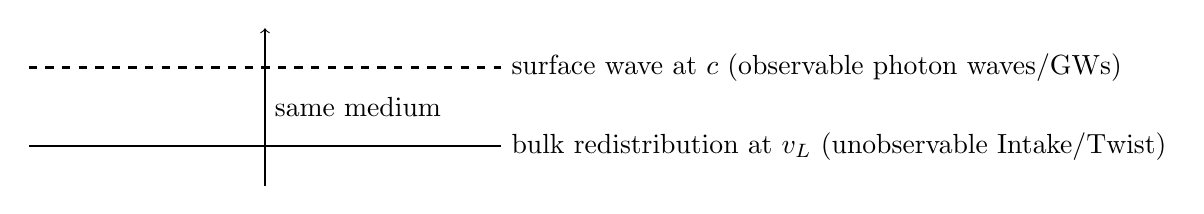
\begin{tikzpicture}
\draw[thick] (0,0) -- (6,0) node[right] {bulk redistribution at $v_L$ (unobservable Intake/Twist)};
\draw[thick,dashed] (0,1) -- (6,1) node[right] {surface wave at $c$ (observable photon waves/GWs)};
\draw[->] (3,-0.5) -- (3,1.5) node[midway,right] {same medium};
\end{tikzpicture}

\subsubsection{Dimensional Conventions}
\paragraph{Units and Conventions (EM).} Unless stated otherwise we use Gaussian--cgs units for the electromagnetic field equations and keep $c$ explicit. Thus $\partial_\nu F^{\mu\nu} = (4\pi/c)\, J^\mu$ (Gaussian) $\equiv \mu_0 J^\mu$ (SI). Where $\epsilon$ and $\mu$ appear (e.g., $c = 1/\sqrt{\epsilon\mu}$) they denote effective medium parameters; in Gaussian vacuum set $\epsilon=\mu=1$. When $4\pi$ or $\mu_0,\epsilon_0$ appear elsewhere they refer to the corresponding form of the same relation; we avoid mixing forms within a single derivation.

\paragraph{Speed glossary.} $v_L$ --- bulk aether drift speed (unobservable in local experiments); $c$ --- surface wave speed in the wave sector (observable, fundamental limit); $v_{\text{eff}}$ --- local effective wave speed set by medium parameters when discussing dispersion. Note: $v$ is always the source/observer speed on the slice; $v_L$ never appears in observables except as a separation-of-scales assumption.

\paragraph{Units and normalization.} Unless otherwise noted we set $\hbar=m=1$ and reinstate them when needed for clarity; all formulas are consistent with this choice.

\paragraph{Projection rules (explicit).} We project along the transverse coordinate $w$ with a slab window $\chi(w)$ of width $\sim\xi_c$ (normalized: $\int\chi(w)\,dw=1$):
\[
\rho_{3D}(\mathbf x,t)=\int \rho_{4D}(\mathbf x,w,t)\,\chi(w)\,dw,\qquad
\int\delta^4(\mathbf r_4-\mathbf r_{4,i})\,dw=\delta^3(\mathbf r-\mathbf r_i).
\]
This fixes all 4D$\to$3D dimensions (e.g., $\rho_0=\rho_{4D}^0\,\xi_c$).

\begin{tcolorbox}[title=Units cheat sheet,colback=gray!5,colframe=gray!35!black]
\begin{tabularx}{\linewidth}{@{}l l X@{}}
Symbol & Units & Description \\
\hline
$\rho_{4D}$ & $M L^{-4}$ & Bulk density \\
$\rho_{3D}$ & $M L^{-3}$ & Projected density ($\rho_{3D}=\int \rho_{4D}\,dw$) \\
$\Gamma$ & $L^{2} T^{-1}$ & Sheet strength (circulation) \\
$\dot M_i$ & $M T^{-1}$ & Sink/source rate at intersection $i$ \\
$\Psi$ & $L^{-2}$ & Surface-like scalar potential (from projection) \\
$\mathbf A$ & $L^{-1}$ & Projected vector potential (unit choice: HL units) \\
$F_{\mu\nu}$ & $T^{-1}$ & Field strength (with $c=1$ convention) \\
$v_L,\,c$ & $L T^{-1}$ & Bulk equilibration vs. observable wave speed \\
\end{tabularx}
\end{tcolorbox}

The $4D\to3D$ projection of codimension-2 defects necessitates non-standard dimensions for the order parameter $\Psi$. This is not an arbitrary choice but a mathematical requirement:

\textbf{Why $[\Psi] = [L^{-2}]$ is necessary:}
\begin{enumerate}
\item In 4D: vortices are 2D sheets (codimension-2 defects)
\item Surface-like fields naturally scale as $[L^{-2}]$
\item Projection to 3D points requires this scaling for consistency
\item Standard 3D conventions $[M^{1/2} L^{-3/2}]$ fail at vortex intersections
\end{enumerate}

Note that this differs from the standard 3D GP scaling of $[L^{-3/2}]$ (or with mass $[M^{1/2} L^{-3/2}]$), as it reflects the codimension-2 defects in 4D appearing surface-like, ensuring consistent projection to 3D points without extraneous mass dimensions. This choice is verified dimensionally in Table \ref{tab:notation} and supports the spine modes, e.g., core Twist/Eddies projecting to EM and Drag's circulation.

This unconventional choice ensures dimensional consistency throughout the projection mechanism (detailed in Section 2.7) and has been verified through comprehensive symbolic analysis.

\medskip

The postulates are summarized in the following table:

We will also use the cosmological length scale $\lambda_{\text{cosmo}}$, tied to large-scale matter distribution and bulk-mode dissipation.

\begin{table}[H]
\centering
\small
\begin{tabularx}{\textwidth}{|c|X|X|X|X|}
\hline
\# & Verbal Statement & Mathematical Input & Quintet Mode & Physical Picture \\
\hline
\textbf{P-1} & Compressible 4D medium with GP dynamics & Continuity: $\partial_t \rho_{4D} + \nabla_4 \cdot (\rho_{4D} \mathbf{v}_4) = 0$ Euler: $\partial_t \mathbf{v}_4 + (\mathbf{v}_4 \cdot \nabla_4) \mathbf{v}_4 = -(1/\rho_{4D}) \nabla_4 P$ Barotropic EOS: $P = (g/2) \rho_{4D}^2 / m$ & Intake/Twist-dominant & Compressible superfluid; defects = holes where phase winds \\
\hline
\textbf{P-2} & Vortex sinks drain into extra dimension & Sink term: $-\sum_i \dot{M}_i \delta^4(\mathbf{r}_4 - \mathbf{r}_{4,i})$ Sink strength: $\dot{M}_i = \rho_{4D}^0 \Gamma_i \xi_c^2$ & Intake & Cores = tiny drains into ±w; no depletion on slice \\
\hline
\textbf{P-3} & Dual wave modes (bulk $v_L$, vortex oscillations $c$) & Longitudinal: $v_L = \sqrt{g \rho_{4D}^0 / m}$ Transverse: $c$ emergent from vortex dynamics Effective: $v_{\text{eff}} = \sqrt{g \rho_{4D}^{\text{local}} / m}$ & Waves (with Intake/Twist in the bulk) & Bulk re-equilibrates quietly; surface waves = photons \\
\hline
\textbf{P-4} & Helmholtz decomposition on the slice (Slope potential + Eddies solenoidal), with Intake across the slab & $\mathbf{v}_4 = -\nabla_4 \Phi + \nabla_4 \times \mathbf{B}_4$ & Slope + Eddies/Drag & Local donut slice around sheet gives textbook $1/\rho$ swirl \\
\hline
\textbf{P-5} & Projection invariance of circulation & Circulation: $\Gamma = n \kappa$, $\kappa = 2 \pi \hbar / m$; slice loop linking once measures $\Gamma$; half-spaces contribute $\Gamma/2$ each; potential fields contribute zero. Vortices as tori/sheets with \textbf{Twist} (quantized cross-slab circulation; $\theta+\tau w$) & Eddies/Drag (with Waves) & Any loop linking once reads same $\Gamma$, regardless of slab thickness \\
\hline
\textbf{P-6} & Discrete vortex projection & Projection: $\sum_i$ not $\int dw$ Vortices intersect at points: $\{(\mathbf{r}_i, w_i)\}$ Observable quantities aggregate discretely & All modes (projection) & Sheets pierce slice at points--count them, don't average \\
\hline
\end{tabularx}
\caption{Foundational postulates presented as mathematical axioms.}
\label{tab:postulates}
\end{table}

For clarity and dimensional consistency, we define the following key quantities. All projections incorporate the healing length $\xi$ to bridge 4D and 3D descriptions. We define the summation operator over projected quantities in the discrete limit, where $i$ indexes vortex intersections. Surface terms vanish in the discrete projection, as there are no infinite boundaries.

\begin{table}[H]
\centering
\begin{tabularx}{\textwidth}{|l|Y|l|l|}
\hline
Symbol & Description & 4D (Pre-Projection) & 3D (Post-Projection) \\
\hline
$\rho_{4D}$ & True 4D bulk density & $[M L^{-4}]$ & --- \\
\hline
$\rho_{3D}$ & Projected 3D density & --- & $[M L^{-3}]$ \\
\hline
$\rho_0$ & 3D background density, defined as $\rho_0 = \rho_{4D}^0 \xi_c$ & --- & $[M L^{-3}]$ \\
\hline
$\rho_{\text{body}}$ & Effective matter density from aggregated deficits & --- & $[M L^{-3}]$ \\
\hline
$g$ & Gross-Pitaevskii interaction parameter & $[L^6 T^{-2}]$ & $[L^6 T^{-2}]$ \\
\hline
$P$ & 4D pressure & $[M L^{-2} T^{-2}]$ & --- \\
\hline
$\xi_c$ & Core healing length (fundamental drainage scale) & $[L]$ & $[L]$ \\
\hline
$\xi_h$ & Twist scale (electromagnetic interaction scale) & $[L]$ & $[L]$ \\
\hline
$v_L$ & Bulk sound speed, $v_L = \sqrt{g \rho_{4D}^0 / m}$ & $[L T^{-1}]$ & --- \\
\hline
$v_{\text{eff}}$ & Effective local sound speed, $v_{\text{eff}} = \sqrt{g \rho_{4D}^{\text{local}} / m}$ & $[L T^{-1}]$ & $[L T^{-1}]$ \\
\hline
$c$ & Emergent light speed (vortex modes) & --- & $[L T^{-1}]$ \\
\hline
$\Gamma$ & Quantized circulation & $[L^2 T^{-1}]$ & $[L^2 T^{-1}]$ \\
\hline
$\kappa$ & Quantum of circulation, $\kappa = 2 \pi \hbar / m$ & $[L^2 T^{-1}]$ & $[L^2 T^{-1}]$ \\
\hline
$\dot{M}_i$ & Sink strength at vortex core $i$, $\dot{M}_i = \rho_{4D}^0 \Gamma_i \xi_c^2$ & $[M T^{-1}]$ & --- \\
\hline
$m$ & Boson mass in Gross-Pitaevskii equation & $[M]$ & $[M]$ \\
\hline
$\hbar$ & Reduced Planck's constant (for quantum terms) & $[M L^2 T^{-1}]$ & $[M L^2 T^{-1}]$ \\
\hline
$G$ & Newton's gravitational constant, calibrated as $G = c^2 / (4\pi \bar{n} \bar{m} \xi_c^2)$ & --- & $[M^{-1} L^3 T^{-2}]$ \\
\hline
$\chi$ & Scalar velocity potential (irrotational Intake flow component), with $\mathbf v=\nabla\chi$ & $[L^2 T^{-1}]$ & --- \\
\hline
$\Phi_g$ & Gravitational potential (weak-field sector) & --- & $[L^2 T^{-2}]$ \\
\hline
$\mathbf{B}_4$ & Vector velocity potential (solenoidal Eddies/Drag flow component) & $[L^2 T^{-1}]$ & --- \\
\hline
$\Psi$ & GP order parameter & $[L^{-2}]$ & --- \\
\hline
$\mathbf{A}_{\text{EM}}$ & Electromagnetic vector potential on the slice (Eddies vector potential) & --- & $[L T^{-1}]$ \\
\hline
$\bar{n}$ & Vortex density (number per unit volume) & $[L^{-3}]$ & $[L^{-3}]$ \\
\hline
$\bar{m}$ & Average deficit mass per vortex & $[M]$ & $[M]$ \\
\hline
$\tau$ & Twist density along extra dimension & $[L^{-1}]$ & $[L^{-1}]$ \\
\hline
$\omega$ & Kelvin wave frequency for wave-sector modes & $[T^{-1}]$ & $[T^{-1}]$ \\
\hline
$\lambda_{\text{cosmo}}$ & Cosmological scale (Hubble-like length; sets dissipation horizon and Machian balance) & $[L]$ & $[L]$ \\
\hline
$\Pi$ & Observation slice $\{w=0\}\subset\mathbb{R}^4$ & --- & --- \\
\hline
$\Sigma$ & Vortex sheet (codimension-2) in $\mathbb{R}^4$ & --- & --- \\
\hline
$w$ & Extra-dimension coordinate (normal to $\Pi$) & $[L]$ & --- \\
\hline
$\gamma$ & Closed loop in $\Pi$ linking $\Sigma\cap\Pi$ & --- & --- \\
\hline
$\rho$ & Loop radius in $\Pi$ (for $v_\theta(\rho)$, circulation loops) & $[L]$ & $[L]$ \\
\hline
$\mathcal{K}$ & Local curvature scale of $\Sigma$ (thin/flat uses $\mathcal{K}\rho\ll1$) & $[L^{-1}]$ & $[L^{-1}]$ \\
\hline
$\mathbf{v}$ & Velocity field (restricts to $\Pi$ for observables) & $[L T^{-1}]$ & $[L T^{-1}]$ \\
\hline
$\phi\ (\equiv \Phi_{\text{Slope}})$ & Slice Slope (electric) potential on $\Pi$ (Helmholtz gradient piece) & --- & $[L^2 T^{-2}]$ \\
\hline
\end{tabularx}
\caption{Key quantities, their descriptions, and dimensions. All projections incorporate the healing length $\xi_c$ for dimensional consistency between 4D and 3D quantities. Dimensions distinguish core-specific quantities from bulk parameters. Polarization emerges from aligned extensions into the extra dimension $w$ for wave-sector stability, yielding two observable polarizations in 3D projections.}
\label{tab:notation}
\end{table}
\paragraph{Notation and conventions.}
We adopt metric signature $(-,+,+,+)$ unless stated otherwise.
The electromagnetic four-potential is $A^\mu_{\text{EM}}=(\Phi_{\text{Slope}}/c,\mathbf A_{\text{EM}})$, with $A_{\mu}^{\text{EM}} = (-\Phi_{\text{Slope}}/c,\mathbf A_{\text{EM}})$ (\emph{Eddies vector potential}) on the slice. For healing lengths, we spell out $\xi_c$ (core/drainage) and $\xi_h$ (Twist/EM). Densities labeled $\rho_0$ are 3D background densities: $\rho_0 := \rho_{3D}^0$.

\subsubsection{Derivation from Aether Dynamics}

From the foundational postulates (P-1 through P-6), we derive the unified field equations governing the dynamics of the 4D compressible superfluid aether. The equations separate into scalar (Intake), vector (Eddies/Drag), and time-dependent pieces (Slope/Induction and Waves), with EM emerging on the slice via Eddies organized by Drag and a hidden core Twist. We begin with the continuity and Euler equations (P-1), incorporating vortex sinks (P-2) and dual wave modes (P-3). Using Helmholtz decomposition (P-4), we separate the velocity field into irrotational (scalar $\Phi_g$ $[L^2 T^{-2}]$) and solenoidal (vector $\mathbf{B}_4$ $[L^2 T^{-1}]$) components, with quantized circulation and core Twist (P-5) providing sources. The dynamics naturally separate into Intake (scalar), Eddies/Drag (solenoidal), and propagating Waves with Slope/Induction, as detailed below. While we reference these modes intuitively in the text, the mathematics uses standard notation without complex quintet forms.

The derivation begins with the 4D equations from P-1 and P-2, now coupled to the vortex core condition $\Psi=0$ at the defect position, incorporating helical twists:

\begin{equation}
\partial_t \rho_{4D} + \nabla_4 \cdot (\rho_{4D} \mathbf{v}_4) = -\sum_i \dot{M}_i \delta^4(\mathbf{r}_4 - \mathbf{r}_{4,i}),
\end{equation}

where $\rho_{4D}$ is the 4D density $[M L^{-4}]$, $\mathbf{v}_4$ the 4-velocity, and $\dot{M}_i = \rho_{4D}^0 \Gamma_i \xi_c^2$ the sink strength (P-2), with the delta supported on the vortex sheet.

\textit{Physically:} Density piles up along ±w; on the slice this looks like Intake only.

The Euler equation is:

\begin{equation}
\partial_t \mathbf{v}_4 + (\mathbf{v}_4 \cdot \nabla_4)\,\mathbf{v}_4
= -\,\frac{1}{\rho_{4D}}\,\nabla_4 P \;-\; \nabla_4 Q_{\rm reg}(\rho_{4D})\,,
\end{equation}

with barotropic EOS $P=\tfrac{g}{2}\,\rho_{4D}^2/m$. Here, $m$ is the effective boson mass in the GP description, ensuring $[P]=[M L^{-2}T^{-2}]$ with $[g]=[L^6T^{-2}]$ and $[\rho_{4D}]=[M L^{-4}]$ (yielding local effective speed $v_{\text{eff}}=\sqrt{g\,\rho_{4D}^{\text{local}}/m}$; bulk $v_L=\sqrt{g\,\rho_{4D}^0/m}$ potentially $\gg c$; observable modes at $c$ from P-3). The term $Q_{\rm reg}$ denotes a short-wavelength \emph{dispersive} (Bogoliubov/GP-type) pressure used only for core-scale regularization at lengths $\sim\xi_c$; its slice-level (Madelung) form and interpretation are developed in Sec.~\ref{sec:QM_projection}.

\textit{Physically:} Pressure gradient reshapes Slope; quantum pressure stiffens the rim.

Helical twists from P-5 introduce a chiral term in the vorticity: $\nabla_4 \times \mathbf{v}_4 = \Omega_0 + (\tau c) \mathbf{n}$ (twist density $\tau$ for the hidden \emph{Twist}, sourcing EM currents preliminarily; normal to vortex $\mathbf{n}$, scaled by $c$ for observable shear; enables Drag). The vorticity $\nabla_4 \times \mathbf{v}_4 = \Omega_0 + (\tau c) \mathbf{n}$ arises from P-5 phase windings $\theta = n\phi + \tau w$, where $\tau$ sources EM currents (detailed in 2.3).

Linearize around background $\rho_{4D} = \rho_{4D}^0 + \delta \rho_{4D}$, $\mathbf{v}_4 = \mathbf{0} + \delta \mathbf{v}_4$ (steady state), and vortex perturbation $\delta R$. The linearized continuity is:

\begin{equation}
\partial_t \delta \rho_{4D} + \rho_{4D}^0 \nabla_4 \cdot \delta \mathbf{v}_4 = -\sum_i \dot{M}_i \delta^4(\mathbf{r}_4 - \mathbf{r}_{4,i}),
\end{equation}

The linearized Euler (dropping quadratic terms):

\begin{equation}
\partial_t \delta \mathbf{v}_4 = -v_{\text{eff}}^2 \nabla_4 (\delta \rho_{4D} / \rho_{4D}^0) - \nabla_4 \delta Q,
\end{equation}

where $\delta P = v_{\text{eff}}^2 \delta \rho_{4D}$ from EOS linearization (differentiate $P(\rho_{4D})$ at $\rho_{4D}^0$ gives $\partial P / \partial \rho_{4D} = g \rho_{4D}^0 / m = v_L^2$, local $\rho_{4D}^{\text{local}}$ for $v_{\text{eff}}$ near deficits), and $\delta Q$ the perturbation in quantum pressure. This separation highlights Intake in density perturbations and Eddies/Drag in vorticity sources.

The vortex dynamics, derived from varying the GP functional with boundary $\Psi=0$ on the defect, yield Kelvin wave equations for oscillations:

\begin{equation}
\partial^2 R / \partial t^2 = c^2 \nabla^2 R + f_{\text{bulk}} + \omega^2 \delta R,
\end{equation}

where the bulk coupling term follows from the defect advecting with the local flow (motivated by superfluid vortex dynamics in P-1 and P-5), $c$ is the emergent speed for Kelvin modes (calibrated, independent of $v_L$), and the oscillatory term $\omega^2 \delta R$ provides harmonic restoring force for near-rim Slope stability, with $\omega \sim v_L / \xi_c$.

\textit{Physically:} Rim oscillations = photons; off-resonance energy leaks as radiation.

Apply Helmholtz decomposition (P-4) to $\delta \mathbf{v}_4 = -\nabla_4 \Phi_g + \nabla_4 \times \mathbf{B}_4$, separating compressible (scalar $\Phi_g$ $[L^2 T^{-2}]$) and incompressible (vector $\mathbf{B}_4$ $[L^2 T^{-1}]$) parts, now with oscillatory modulation in the phase. Taking $\nabla_4 \cdot$ on Euler gives:

\begin{equation}
\partial_t (\nabla_4 \cdot \delta \mathbf{v}_4) = -v_{\text{eff}}^2 \nabla_4^2 (\delta \rho_{4D} / \rho_{4D}^0) - \nabla_4^2 \delta Q,
\end{equation}

and substituting $\nabla_4 \cdot \delta \mathbf{v}_4 = -\nabla_4^2 \Phi_g$ yields the scalar precursor. From linearized continuity:

\begin{equation}
\nabla_4 \cdot \delta \mathbf{v}_4 = -\frac{1}{\rho_{4D}^0} \left( \partial_t \delta \rho_{4D} + \sum_i \dot{M}_i \delta^4(\mathbf{r}_4 - \mathbf{r}_{4,i}) \right).
\end{equation}

Differentiate continuity by $t$:

\begin{equation}
\partial_{tt} \delta \rho_{4D} + \rho_{4D}^0 \partial_t (\nabla_4 \cdot \delta \mathbf{v}_4) = -\sum_i \partial_t \dot{M}_i \delta^4(\mathbf{r}_4 - \mathbf{r}_{4,i}),
\end{equation}

and substitute the Euler divergence:

\begin{equation}
\partial_{tt} \delta \rho_{4D} - \rho_{4D}^0 v_{\text{eff}}^2 \nabla_4^2 (\delta \rho_{4D} / \rho_{4D}^0) = -\sum_i \partial_t \dot{M}_i \delta^4(\mathbf{r}_4 - \mathbf{r}_{4,i}) + \rho_{4D}^0 \nabla_4^2 \delta Q.
\end{equation}

Combine with $\nabla_4 \cdot \delta \mathbf{v}_4 = -\nabla_4^2 \Phi_g$:

\begin{equation}
\partial_{tt} \Phi_g - v_{\text{eff}}^2 \nabla_4^2 \Phi_g = v_{\text{eff}}^2 \sum_i \frac{\dot{M}_i}{\rho_{4D}^0} \delta^4(\mathbf{r}_4 - \mathbf{r}_{4,i}) + v_{\text{eff}}^2 \nabla_4^2 \delta Q / \rho_{4D}^0.
\end{equation}

\begin{tcolorbox}[title=Dimensional Checks]
Dimensions for continuity: LHS $[\partial_t \rho_{4D}] = [M L^{-4} T^{-1}]$, $[\nabla_4 \cdot (\rho_{4D} \mathbf{v}_4)] = [M L^{-4} T^{-1}]$, RHS $[\dot{M}_i \delta^4] = [M T^{-1}] [L^{-4}] = [M L^{-4} T^{-1}]$.

Dimensions for Euler: LHS $[\partial_t \mathbf{v}_4] = [L T^{-2}]$, $[(\mathbf{v}_4 \cdot \nabla_4) \mathbf{v}_4] = [L T^{-2}]$, RHS $[\nabla_4 P / \rho_{4D}] = [M L^{-2} T^{-2}] [M^{-1} L^{4}] = [L T^{-2}]$.
\end{tcolorbox}

\begin{tcolorbox}
The aether determines HOW FAST disturbances propagate locally, not WHERE they propagate from.
\end{tcolorbox}


\subsubsection{Scalar Sector: Gravitational Attraction}

\textbf{What you'd measure:} Gravimeter sees $\nabla\Phi_g$ from Intake; redshift as energy stored in Slope. Test masses fall toward cores as deficit regions need filling.

This sector corresponds to pure Intake: irrotational flow ($\nabla \times \mathbf{v} = 0$) creating attractive pressure gradients, analogous to the cavity-filling rush of water in the tsunami analogy (inward flow to fill density deficits). This ties to particles as processes: mass emerges from the deficit volume in stable flow patterns around vortices. Contrast with the EM sector (2.3), where sources include on-slice Eddies (organized by Drag) with a hidden core Twist at rest.

\subsubsection{Vector Sector: Eddies (B) and Drag Effects}

\textbf{What you'd measure:} Moving core drags medium; on-slice map is B-like whirl patterns circling motion. Compass needles align with eddies; charged particles spiral.

Eddies are the on-slice circulation (magnetic) organized by Drag (motion of linked cores). A tiny, hidden Twist at rest gives only a $1/r^3$ dipole; bulk motion dominates the observable $\mathbf B$. For the vector sector, vorticity $\nabla \times \mathbf{v} = \boldsymbol{\omega}$ is sourced by moving vortices (P-5).

For electromagnetism, keep the electromagnetic potential distinct as $\mathbf A_{\text{EM}}$ for currents driven by Eddies (Eddies vector potential). For the EM wave equations and charge/current continuity, see Sec.~\ref{sec:EM_projection}.

\subsubsection{Slope (Coulomb) and Waves}

\textbf{What you'd measure:} Static hill/valley stores energy; modulate the rim → loop-E induction, radiative escape. Voltmeters read potential differences; antennas detect wave ripples.

Slope (static hill/valley electric piece) and the wave sector (photons for EM). In time-varying situations, changing Eddies create loop electric fields (Induction). Wave equations and retarded solutions for EM are developed in Sec.~\ref{subsec:em_wave}. The tsunami principle distinguishes bulk longitudinal adjustments ($v_L > c$, unobservable Intake/Twist) from observable transverse waves at $c$ in the wave sector, with the wave sector as the surface ripple versus bulk Intake rush. To derive these, consider the linearized GP for transverse perturbations on vortices: The Kelvin wave dispersion $\omega^2 = c^2 k^2 + \omega_0^2$ (with cutoff $\omega_0 \sim v_L / \xi_c$), projecting to the d'Alembertian form for far-field radiation.

The near-rim Slope sets the stored energy and shape, while the hidden Twist supplies the hoop (keep-open) pressure; together they stabilize the core against tension and Intake. Annihilation releases $2mc^2$ as radiation in the wave sector. Depletion ($\rho \to 0$) mismatches resonance, causing photon escape and instability.

\subsubsection{Field equations on the slice: sketch and summary}
\label{sec:field-eqs-framework}

Starting from the 4D continuity/Euler system (P–1–P–2), we linearize about the steady background, apply a Helmholtz split to the perturbation, and project through the slab window $\chi(w)$. Codimension and discrete intersections fix the 4D$\!\to$3D units. On the slice $\Pi$ this yields a scalar intake potential $\Psi$ (irrotational, speed $v_{\text{eff}}$) and a vector eddy potential $\mathbf A$ (solenoidal, speed $c$); sources close by sink content and quantized circulation/defect motion (with twist contributions). The heavy derivations and gauges live in the split papers.

\begin{tcolorbox}
\textbf{Key equations on the slice $\Pi$.}

\noindent\textbf{Scalar (Intake):}
\begin{equation}
\frac{1}{v_{\text{eff}}^{2}}\partial_{tt}\Psi - \nabla^{2}\Psi = \mathcal S_{\Psi}.
\label{eq:scalar-fw}
\end{equation}

\noindent\textbf{Vector (Eddies):}
\begin{equation}
\frac{1}{c^{2}}\partial_{tt}\mathbf A - \nabla^{2}\mathbf A = \boldsymbol{\mathcal S}_{A}.
\label{eq:vector-fw}
\end{equation}

\noindent\textbf{Eddy fields \& identities:}
\begin{subequations}\label{eq:eddy-block}
\begin{align}
\mathbf B_{\text{eddy}} &:= \nabla\times\mathbf A,
&
\mathbf E_{\text{eddy}} &:= -\,\partial_t \mathbf A,
\label{eq:eddy-fields}
\\
\nabla\!\cdot\!\mathbf B_{\text{eddy}} &= 0,
&
\nabla\times\mathbf E_{\text{eddy}}+\partial_t \mathbf B_{\text{eddy}} &= 0.
\label{eq:homogeneous-eddy}
\end{align}
\end{subequations}

\noindent\textit{Sources}: $\mathcal S_{\Psi}$ from projected sink strength;
$\boldsymbol{\mathcal S}_{A}$ from quantized circulation/defect motion (twist-coupled).

\medskip
\noindent\textbf{Physical cheat-map:}
\begin{center}
\begin{tabularx}{\linewidth}{|l|l|X|}
\hline
\textbf{Math Symbol} & \textbf{Physical Name} & \textbf{What it means} \\
\hline
$\mathbf{E}_{\text{slope}}$ & Slope & Standing hill/valley pattern from oriented links (Coulomb $\mathbf{E}$) \\
\hline
$\mathbf{E}_{\text{loop}}$ & Induction & Ring-shaped electric push when eddies change (Faraday $\mathbf{E}$) \\
\hline
$\mathbf{B}_{\text{eddy}}$ & Eddies & On-slice whirls with no loose ends (magnetic field) \\
\hline
\end{tabularx}
\end{center}
\end{tcolorbox}

\paragraph*{Notes \& pointers.}
Gravity/GEM: Lorenz gauge, Maxwell-like set, potential waves, force law (\S\ref{sec:gauge}, \S\ref{sec:gw-linear}–\S\ref{sec:resummed-dict}).\;
Projected EM: definitions \eqref{eq:EM_defs}, homogeneous \eqref{eq:homogeneous}, closures and $c$ via \eqref{eq:inhomogeneous}, \eqref{eq:c_relation}, \eqref{eq:wave_A_Lorenz}.\;
Quantum: minimal coupling, continuity/current, Madelung \(Q\), KG/Dirac (\S\ref{sec:QM_ops}–\S\ref{sec:QM_madelung_detail}, \eqref{eq:schrodinger}, \eqref{eq:current}–\eqref{eq:continuity}, \eqref{eq:Q_potential}, \eqref{eq:kg}–\eqref{eq:dirac}).



\subsection{Resolution of the Preferred Frame Problem}
\label{subsec:preferred-frame}

\paragraph*{Layering (observables vs.\ micro-mechanics).}
The microscopic medium admits a natural rest frame, but \emph{gauge-invariant observables on the projected 3+1 slice} do not reveal a global preferred frame to leading order. Excitations propagate on an emergent Minkowski sector with limiting speed $c$, and local inertial behavior is set by distributed sources (Mach-type influence) rather than by access to the medium's micro-rest frame.

\paragraph*{Plain-language summary.} The medium in our model could have its own “rest frame,” but none of the \emph{measurable} fields can see it at leading order. The signals our instruments use (light, EM disturbances, weak-field gravity) live on an emergent relativistic surface with a built-in speed limit $c$, so two-way measurements--like Michelson–Morley--come out isotropic and show no ether wind. Any imprint of a background drift would show up only as much smaller, higher-order effects (scaling with the square of the drift speed and other tiny parameters) that cancel or fall below experimental sensitivity. In short: a microscopic current may exist in the deep background, but there's no observable “preferred frame” in the physics you can measure.

\paragraph{Conventions and scope.}
(1) We use signature $\eta_{\mu\nu}=\mathrm{diag}(-,+,+,+)$ and Greek indices $\mu,\nu=0,\dots,3$.
(2) Electromagnetic-like observables are built from a \emph{single} vector potential $A^\mu=(\Phi_{\text{Slope}}/c,\mathbf A)$ with field strength $F_{\mu\nu}=\partial_\mu A_\nu-\partial_\nu A_\mu$.
(3) If a gravito-electromagnetic sector is also considered, we denote its vector potential distinctly (e.g.\ $\mathcal A^\mu$) or use metric perturbations $h_{\mu\nu}$; we do \emph{not} overload $A^\mu$.
(4) EM unit conventions and Maxwell’s equations are developed in Sec.~\ref{sec:EM_projection}. Here we only fix notation for the field strength $F_{\mu\nu}=\partial_\mu A_\nu-\partial_\nu A_\mu$.
(5) Small parameters controlling all approximations:
\begin{equation}
\varepsilon_v=\frac{|\mathbf v_{\rm bg}|}{c},\qquad
\varepsilon_{\Phi_g}=\frac{|\Phi_g|}{c^2},\qquad
\varepsilon_\xi=\frac{\xi_c}{L},\qquad
\varepsilon_\rho=\frac{\delta\rho}{\rho_0}.
\end{equation}
Claims below hold at leading order in $(\varepsilon_{\Phi_g},\varepsilon_v^2,\varepsilon_\xi,\varepsilon_\rho)$ unless noted.

\paragraph{Field equations, covariance, and invariants.}
On the observed slice, the Lorenz-gauge system
\begin{equation}
\Box A^\mu = -\frac{4\pi}{c}\,J^\mu,\qquad \partial_\mu A^\mu=0,
\end{equation}
is Lorentz covariant: under a standard boost (say along $x$) the components of $A^\mu$ mix as in special relativity, and the scalars
\begin{equation}
\mathcal I_1 = F_{\mu\nu}F^{\mu\nu}=2\,(B^2-E^2/c^2),\qquad
\mathcal I_2 = {}^\star\!F_{\mu\nu}F^{\mu\nu}=-\frac{4}{c}\,\mathbf E\cdot\mathbf B
\end{equation}
are frame-invariant. Observable content is therefore independent of any putative medium drift. Causal support follows from the retarded Green's function of $\Box$ (see the appendix discussion of retarded kernels in higher spatial dimension): signal propagation is restricted to the $c$-lightcone, and static Poisson behavior is a limit of the retarded solution.

\paragraph{No observable ``ether wind'' at leading order.}
Preferred-frame effects can enter (if at all) only through (i) gauge/constraint pieces that cancel in $F_{\mu\nu}$, (ii) post-projection finite-thickness corrections $\mathcal O(\varepsilon_\xi)$, (iii) nonlinear backreaction $\mathcal O(\varepsilon_{\Phi_g})$, or (iv) quadratic drift effects $\mathcal O(\varepsilon_v^2)$. None of these produce a first-order ($\propto \varepsilon_v$) anisotropy in any gauge-invariant observable.

\paragraph{Michelson–Morley as a worked test.}
Consider an interferometer with equal arm lengths $L$ oriented parallel/perpendicular to a putative background drift $\mathbf v_{\rm bg}$. In the emergent Minkowski sector the measured (two-way) light speed is isotropic to $\mathcal O(\varepsilon_v^2)$, and the round-trip times are
\begin{equation}
t_{\parallel}=\frac{2L}{c}\Big(1+\tfrac{1}{2}\beta^2\Big)+\mathcal O(\varepsilon_{\Phi_g},\varepsilon_\xi,\beta^4),\qquad
t_{\perp}=\frac{2L}{c}\Big(1+\tfrac{1}{2}\beta^2\Big)+\mathcal O(\varepsilon_{\Phi_g},\varepsilon_\xi,\beta^4),
\end{equation}
with $\beta\equiv|\mathbf v_{\rm bg}|/c$. The leading $\beta^2$ pieces cancel in the time \emph{difference},
\begin{equation}
\Delta t \equiv t_{\parallel}-t_{\perp}=\mathcal O(\varepsilon_{\Phi_g},\varepsilon_\xi,\beta^4),
\end{equation}
so the predicted fringe shift is null at the experiment's sensitivity scale--precisely as in special relativity. The same cancellation holds for modern resonator tests of boost/rotation invariance at this order.

\textbf{Worked number:} For the historical Michelson-Morley setup with $L = 11$ m and Earth's orbital speed $\beta \sim 10^{-4}$:
\begin{align*}
\Delta t &= t_{\parallel} - t_{\perp} \sim \frac{2L}{c} \cdot \beta^4 \\
&\sim \frac{2 \times 11\text{ m}}{3 \times 10^8\text{ m/s}} \times (10^{-4})^4 \\
&\sim 7 \times 10^{-8}\text{ s} \times 10^{-16} \sim 10^{-23}\text{ s}
\end{align*}
This is far below the $\sim 10^{-16}$ s resolution of the original experiment, confirming null result.

\paragraph{What the framework \emph{does} and \emph{does not} predict.}
At leading order the observable sector exhibits: (i) Lorentz-covariant dynamics with characteristic speed $c$, (ii) isotropy of two-way light speed, and (iii) no direction-dependent variation of effective couplings. Slow secular drifts of global background parameters, if present, would appear only as higher-order, adiabatic effects beyond the scope of this subsection and are not required by the framework.

\paragraph{Summary.}
The microscopic medium can possess a rest frame without violating relativity tests, because the projected, gauge-invariant fields $(F_{\mu\nu}$ and, analogously, $h_{\mu\nu}$ in the weak-field sector$)$ satisfy Lorentz-covariant, hyperbolic equations with retarded support. Any ``preferred frame'' is unobservable at leading order; putative effects are suppressed by $(\varepsilon_{\Phi_g},\varepsilon_v^2,\varepsilon_\xi,\varepsilon_\rho)$ and are thus beyond the reach of classic interferometric tests.

\textit{What to picture:} Detectors ride with the bulk reshuffle; only the wavefront at $c$ changes what you see.

\subsection{The Tsunami Principle}

\begin{tcolorbox}[title=Tsunami dictionary,colback=gray!5,colframe=gray!35!black]
\begin{center}
\begin{tabular}{|l|l|l|}
\hline
\textbf{Aspect} & \textbf{Bulk tsunami} & \textbf{Observable wave} \\
\hline
Driver & Vortex core sink/source & Time-varying fields \\
Carrier & Density redistribution & EM/gravity waves \\
Speed & $v_L \gg c$ (unobservable) & $c$ (observable) \\
\hline
\end{tabular}
\end{center}
Key insight: Same medium, different physics--bulk rush vs surface ripple.
\end{tcolorbox}

\textbf{Statement.} Bulk density in the 4D medium can re-equilibrate rapidly at a characteristic speed $v_L$ that never appears in gauge-invariant observables. All measurable fields on the observed 3D slice---e.g., electromagnetic $A_\mu$ with $F_{\mu\nu}$, or metric perturbations $h_{\mu\nu}$---propagate causally with retarded Green's functions at the limiting speed $c$. There is no superluminal signaling: fast \emph{setup} in the bulk is not a signal in the observables.

\medskip
\noindent\textbf{Bulk setup (unobservable).} As a simple model of a sudden local change, consider a pointlike impulse at the origin of the 4D space at $t=0$ driving the linear bulk mode for the density perturbation $\delta\rho$:
\begin{equation}
\partial_t^2 \,\delta\rho(\mathbf r_4,t)\;-\; v_L^2 \,\nabla_4^2 \delta\rho(\mathbf r_4,t)
\;=\; -\,M\,\delta^4(\mathbf r_4)\,\delta'(t)\,,
\label{eq:bulk-tsunami}
\end{equation}
where $\mathbf r_4=(x,y,z,w)$, $\nabla_4^2\!\equiv\!\partial_x^2{+}\partial_y^2{+}\partial_z^2{+}\partial_w^2$, and $\delta'(t)$ is the time derivative of the Dirac delta.\footnote{Units audit: $[\delta^4\delta'(t)]=L^{-4}T^{-2}$ so both sides of \eqref{eq:bulk-tsunami} have units $ML^{-4}T^{-2}$. Using $\delta(t)$ without the derivative would be off by one power of $T^{-1}$.}
The retarded solution is
\begin{equation}
\delta\rho(\mathbf r_4,t)\;=\;M\,G^{\rm ret}_{(4)}(\mathbf r_4,t;v_L)\,,
\end{equation}
with $G^{\rm ret}_{(4)}$ the retarded Green's function for the 4-spatial-D wave operator. In even spatial dimension the support has a “tail” inside the $v_L$ cone; schematically one may write $\delta\rho \sim \Theta(t{-}R/v_L)\,f(R,t)$ with $R=|\mathbf r_4|$ to emphasize causality of the bulk setup. See Appendix: \emph{Retarded Green's function in four spatial dimensions} for the explicit form and discussion of causal support.

\medskip
\noindent\textbf{Observables (causal and retarded).} Gauge-invariant fields measured on the 3D slice obey Lorentz-covariant, hyperbolic equations with characteristic speed $c$. For the EM wave equations and retarded solutions, see Sec.~\ref{subsec:em_wave}.
with the standard conservation law $\partial_\mu J^\mu=0$; for the EM charge current specifically, see Eq.~\ref{eq:slice_continuity} in Sec.~\ref{sec:EM_projection}. We impose an outgoing-wave (Sommerfeld) condition at large $r$ (e.g., $(\partial_r-\tfrac1c\partial_t)(r\psi)\!\to\!0$ for each field component $\psi$), which selects the retarded solutions. The effective wave speed $c$ is calibrated by $c=\sqrt{T/\sigma}$ (see the dimensional conventions section for the definitions of the effective tension $T$ and areal density $\sigma$).

\medskip
\noindent\emph{Idea $\Rightarrow$ Result (bulk).} Solve \eqref{eq:bulk-tsunami} with the retarded Green's function in 4 spatial dimensions. \emph{Result:} the bulk density re-equilibrates causally inside the $v_L$ cone; this adjustment is not itself an observable on the slice.

\noindent\emph{Idea $\Rightarrow$ Result (observables).} Solve \eqref{eq:wave_A_Lorenz} with retarded boundary conditions. \emph{Result:} all gauge-invariant observables respond only after $t\ge r/c$; no information propagates faster than $c$.

\medskip
\noindent\textbf{Static limit and apparent ``instantaneity.''} In the near-zone or slowly varying regime ($\omega r/c\!\ll\!1$), the retarded solutions reduce to their familiar static limits (e.g., Poisson/Coulomb), which \emph{look} instantaneous (quasi-static) but are actually the $t{-}r/c\!\to\!t$ approximation of retarded fields. The rapid bulk equilibration sets the quasi-static background against which these observables evolve; it does not transmit signals.

\medskip
\noindent\textbf{Timeline (causal ordering).}
\begin{itemize}
\item $t< R/v_L$: nothing has changed anywhere.
\item $R/v_L < t < r/c$: the 4D bulk density has adjusted; no change yet in gauge-invariant observables at the 3D location $r$.
\item $t\ge r/c$: observable fields ($F_{\mu\nu}$, $h_{\mu\nu}$, etc.) change; signals arrive and can influence detectors.
\end{itemize}

\medskip
\noindent\textbf{Dictionary (one-liners).} Bulk $\delta\rho$ = unobservable setup at $v_L$; observables = gauge-invariant fields on the slice at $c$; ``tsunami'' = bulk re-equilibration; ``wave'' = what detectors measure.

\medskip
\noindent\textbf{Takeaway.} Two distinct speeds coexist without paradox: $v_L$ governs rapid, unobserved bulk equilibration; $c$ governs the propagation of all observables via retarded, Lorentz-covariant field equations. The former never enables superluminal signaling in the latter.

\subsection{Conservation Laws and Aether Drainage}

The 4D compressible medium (P-1) ensures global conservation laws hold despite local drainage from vortex sinks (P-2), as flux redirects into the extra dimension without loss. This resolves apparent non-conservation in 3D projections (Section 2.7) while maintaining consistency with dual wave modes (P-3) and quantized topology (P-5). The framework derives these laws from the Gross–Pitaevskii structure (P-1), incorporating boundary conditions for vortex sheets. We shift to discrete projections, aggregating over finite vortex intersections rather than continuous integrals over $w$. This simplifies boundary handling while preserving the original global principles. The spine integrates naturally: Intake (drainage) appears as apparent mass removal in 3D but is conserved in 4D via bulk redirection; Twist (topology) preserves invariants like charge through phase windings; Drag conserves angular momentum; Slope stabilizes cores energetically; the wave sector (Kelvin waves) conserves energy by converting to bulk modes or observable radiation (e.g., photons as vortex oscillations).

Drainage $\equiv$ net flux $\Phi = \int \rho \mathbf{v} \cdot \hat{\mathbf{n}} \, dA$ through a hypersurface at $w = \text{const}$. Drainage creates Intake but doesn't deplete the medium, as it draws from the effectively infinite 4D reservoir.

\subsubsection{Global Conservation}
Although the sinks introduce effective inhomogeneities in the 3D equations, the full 4D continuity ensures no net loss once boundary fluxes are included. Starting from the postulates (P-1, P-2), the 4D continuity equation with localized sinks is
\begin{equation}
\partial_t \rho_{4D}+\nabla_4 \!\cdot (\rho_{4D}\mathbf{v}_4)\;=\;-\sum_i \dot{M}_i\,\delta^4(\mathbf{r}_4-\mathbf{r}_{4,i}).
\end{equation}
Integrating over all 4D space and applying Gauss' theorem gives
\begin{equation}
\frac{d}{dt}\!\int \rho_{4D}\,d^4 r\;+\;\oint_{\infty}\rho_{4D}\mathbf{v}_4\!\cdot d\mathbf{S}\;=\;-\sum_i \dot M_i,
\end{equation}
i.e. $dM_{4D}/dt+F_\infty=-\sum_i\dot M_i$ with $F_\infty\equiv\oint_{\infty}\rho_{4D}\mathbf{v}_4\!\cdot d\mathbf{S}$. Two consistent steady-state realizations are possible: (i) \emph{paired sources/sinks} with $\sum_i \dot M_i=0$ and $F_\infty=0$, or (ii) a \emph{quasi-steady throughflow} with $dM_{4D}/dt=0$ and $F_\infty=+\sum_i \dot M_i$ (bulk outflow to the reservoir). Either way, global conservation holds in 4D while the $w=0$ slice exhibits apparent removal.

In the discrete 3D projection (P-6), we aggregate over vortex intersections (no averaging operator), defining
\begin{equation}
\partial_t \rho_{3D} + \nabla \!\cdot (\rho_{3D}\mathbf{v}) = -\sum_i \dot{M}_i\,\delta^3(\mathbf{r}-\mathbf{r}_i).
\end{equation}
Analogous projections apply to the Euler equation, producing effective 3D dynamics with sink sources that appear as mass removal while preserving global conservation in 4D (see Bulk Dissipation below). Physically, this is like discrete underwater drains vanishing water from the surface view, thinning the medium and inducing inflows that mimic attraction. Like a waterfall that never empties the river above, the drainage draws from the 4D structure (reservoir), with re-emergence from bulk modes maintaining balance.

By Noether's theorem, continuous symmetries yield conservation laws. 4D translations preserve total mass–energy when one includes the energy density of non-interacting bulk excitations that carry away the drained flux. Particle creation/annihilation maps to vortex–antivortex processes: creation as pair formation (net drainage balanced), annihilation as conversion of core energy into the wave sector or bulk modes, preserving total 4D energy. Conservation includes: Twist topology preserves charge; Drag conserves angular momentum; Slope stabilizes energy; the wave sector radiates energy.

\subsubsection{Microscopic Drainage Mechanism}
At vortex cores, drainage occurs through phase singularities where the order parameter $\Psi=0$ over the healing length $\xi_c$. The phase winds by $2\pi n$, creating flux into the extra dimension. Near the core, a standard circulation estimate gives
\begin{equation}
v_w \;\approx\; \frac{\Gamma}{2\pi r_4},\qquad r_4=\sqrt{\rho^2+w^2},
\end{equation}
with $\Gamma=n\kappa$ the circulation quanta and $\kappa=2\pi\hbar/m$ (P-1). The total sink strength for each vortex follows from a transverse cross-section integral over the core:
\begin{equation}
\dot M_i \;\approx\; \rho_{4D}^0 \int_{\text{core}} v_w\, dA_\perp
\;\approx\; \rho_{4D}^0\,\frac{\Gamma}{2\pi \xi_c}\,(\pi \xi_c^2)
\;\sim\; \rho_{4D}^0\,\Gamma\,\xi_c^2,
\end{equation}
i.e. dimensionally $[\,\dot M_i\,]=M/T$ with $[\rho_{4D}^0]=M/L^4$, $[\Gamma]=L^2/T$, and $[\xi_c^2]=L^2$. Reconnections act as ``valves,'' releasing flux into bulk modes, with an energy barrier
\begin{equation}
\Delta E \;\approx\; \frac{\rho_{4D}^0\,\Gamma^2\,\xi_c^2}{4\pi}\,\ln\!\left(\frac{L}{\xi_c}\right),
\end{equation}
that suppresses uncontrolled leakage (here $L$ is an outer cutoff).

With helical twists (Section 2.3), drainage couples to charge: twisted vortices have enhanced $\dot M_i \propto \tau\,\Gamma$ (twist density $\tau$), but conservation holds as twists preserve topology during reconnections. Wave-sector vibrations (Kelvin waves) modulate the core, adding a small oscillatory term to $v_w$ ($\delta v_w \sim \omega\,\delta R$), while the time-averaged flux remains $\langle \dot M_i \rangle$ unchanged; the excess energy is carried off as radiation.

\subsubsection{Bulk Dissipation}
To prevent accumulation and back-reaction, the bulk continuity includes a dissipation term that converts directed flux to non-interacting excitations:
\begin{equation}
\partial_t \rho_{\text{bulk}} + \partial_w (\rho_{\text{bulk}} v_w) = -\gamma \rho_{\text{bulk}},
\end{equation}
with rate $\gamma \sim v_L/L_{\text{univ}}$ (a horizon scale $L_{\text{univ}}$), and $v_w=\mathrm{sign}(w)\,v$ representing symmetric outward drainage from the $w=0$ slice (P-2). The scale $v \sim v_L=\sqrt{g\rho_{4D}^0/m}$ emerges from bulk longitudinal modes (P-1), while observables remain confined to Kelvin/wave modes at $c$.

\textbf{Key Idea:} Symmetric outward drainage with dissipation.

Solve piecewise in steady state for the spatial profile (transients decay as $e^{-\gamma t}$):
\begin{itemize}
\item $w>0$: $v\partial_w\rho_{\text{bulk}}=-\gamma\rho_{\text{bulk}}\Rightarrow \rho_{\text{bulk}}(w)=\rho(0^+)\,e^{-w/\lambda}$,
\item $w<0$: $-v\partial_w\rho_{\text{bulk}}=-\gamma\rho_{\text{bulk}}\Rightarrow \rho_{\text{bulk}}(w)=\rho(0^-)\,e^{w/\lambda}=\rho(0^-)\,e^{-|w|/\lambda}$,
\end{itemize}
with $\lambda=v/\gamma$. Assuming symmetry $\rho(0^+)=\rho(0^-)=\rho_{\text{inj}}$, the global solution is
\begin{equation}
\rho_{\text{bulk}}(w,t)=\rho_{\text{inj}}\,e^{-\gamma t}\,e^{-|w|/\lambda},\qquad (w\neq 0).
\end{equation}
At $w=0$, the derivative $\partial_w(\rho_{\text{bulk}} v_w)$ develops a delta function,
\begin{equation}
\partial_w\!\left[\mathrm{sign}(w)\,v\,\rho_{\text{bulk}}\right]
= \mathrm{sign}(w)\,v\,\partial_w\rho_{\text{bulk}} + 2v\,\rho_{\text{inj}}\,\delta(w),
\end{equation}
so the matching condition that closes the model is
\begin{equation}
2v\,\rho_{\text{inj}}\,\delta(w)\;=\;\sum_i \dot M_i\,\delta(w)\,\delta^3(\mathbf r-\mathbf r_i),
\end{equation}
i.e. $\rho_{\text{inj}}$ is fixed by the total injection $\sum_i\dot M_i$ on the slice. With this balance, the background $\rho_{4D}^0$ remains approximately constant and the framework is compatible with tight bounds on time variation, $|\dot G/G|\lesssim 10^{-13}\,\mathrm{yr}^{-1}$; no anisotropy in $G$ is predicted at leading order. Wave-sector energy dissipates similarly, converting to bulk modes or photons, preserving total 4D energy. Twists preserve topology (P-5), conserving charge.

Analogously, this dissipation mimics energy conversion to heat in a vast reservoir, maintaining equilibrium. For twisted vortices (EM context), dissipation preserves charge topology, as windings are conserved invariants.

\subsubsection{Machian Balance}
The uniform background $\rho_0$ sources a quadratic potential term. With the scalar-sector convention $\nabla^2 \Phi_g=-4\pi G\rho_0$,
\begin{equation}
\Phi_g \supset -\frac{2\pi G \rho_0}{3}\,r^2,
\end{equation}
implying
\begin{equation}
\mathbf{a} = -\nabla \Phi_g = \frac{4\pi G \rho_0}{3}\,\mathbf{r}.
\end{equation}
Only potential differences are observable; the quadratic background acts as a gauge-like offset that cancels under global balance. Global inflows from cosmic matter (discrete vortices as flow patterns) provide the counter-term
\begin{equation}
\Phi_{\text{global},g} \approx \frac{2\pi G \langle \rho \rangle}{3}\, r^2,
\end{equation}
cancelling if $\langle \rho_{\text{cosmo}} \rangle = \rho_0$ (aggregate deficits from vortex flows balancing background). Any residual asymmetry would appear as a tiny secular drift of the effective background potential; within our parameter choices it remains below current bounds on $|\dot G/G|$.

Twist adds no net background (neutral on average), preserving the balance. The wave sector (Kelvin waves) contributes a small positive energy density to $\langle \rho \rangle$ (as $\rho_{\text{vib}}/c^2$), but this is microscopic and averages out cosmologically, maintaining equilibrium. The tsunami principle reinforces this: bulk flows are unfelt locally (we move with them), while observable changes propagate at $c$.

\medskip
\makebox[\linewidth][c]{%
\fbox{%
\begin{minipage}{\dimexpr\linewidth-2\fboxsep-2\fboxrule\relax}
\textbf{Key Insight:} Global conservation is maintained by bulk absorption and matched boundary flux, while Machian inertial frames arise from inflow balances, without ontological claims. The spine ties this together: Intake for mass flux, Twist for topological charge, Drag for angular momentum, Slope for energetic stability, the wave sector for radiative energy--each conserved in 4D.
\end{minipage}
}
}
\medskip

\subsection{4D→3D Projection Mechanism}

We now make the projection from the $4$-spatial-D description to effective $3$D dynamics precise. The key points are:
(i) projection is an \emph{integration} over the extra coordinate $w$ (or, equivalently, a \emph{sum} over discrete sheet–slice intersections per P-6);
(ii) gradient (“drainage”) adjustments along $w$ are potential on the slice and contribute \emph{no} loop circulation;
(iii) solenoidal flow projects to the standard $1/\rho$ azimuthal profile with circulation equal to the $4$D sheet strength~$\Gamma$.
Throughout we keep units and distributions explicit: $[\rho_{4D}]=ML^{-4}$, $[\Gamma]=L^2T^{-1}$, $[\dot M_i]=MT^{-1}$.

\paragraph{Start from $4$D continuity with localized sinks.}
From P-1 and P-2,
\begin{equation}
  \partial_t \rho_{4D} + \nabla_4\!\cdot(\rho_{4D}\,\mathbf v_4)
  \;=\; -\sum_i \dot M_i\,\delta^4(\mathbf r_4-\mathbf r_{4,i}),
  \label{eq:4D_continuity_projection_start}
\end{equation}
where $\delta^4(\mathbf r_4-\mathbf r_{4,i})=\delta^3(\mathbf r-\mathbf r_i)\,\delta(w-w_i)$ and, for slice intersections, $w_i=0$.
Integrating \eqref{eq:4D_continuity_projection_start} over $w\in\mathbb R$ gives
\begin{equation}
  \partial_t \rho_{3D} + \nabla\!\cdot \mathbf J_{3D}
  \;=\; -\sum_i \dot M_i\,\delta^3(\mathbf r-\mathbf r_i)
  \quad \text{provided}\quad
  [\,\rho_{4D} v_w\,]_{-\infty}^{+\infty}=0,
  \label{eq:3D_continuity_effective}
\end{equation}
with the projected fields defined by
\begin{equation}
  \rho_{3D}(\mathbf r,t)\;=\!\!\int_{-\infty}^{\infty}\!\! \rho_{4D}(\mathbf r,w,t)\,dw,
  \qquad
  \mathbf J_{3D}(\mathbf r,t)\;=\!\!\int_{-\infty}^{\infty}\!\! \rho_{4D}(\mathbf r,w,t)\,\mathbf v_{\!\parallel}(\mathbf r,w,t)\,dw,
  \label{eq:projection_map_defs}
\end{equation}
where $\mathbf v_{\!\parallel}$ is the component tangent to the slice. If one prefers an explicit finite-thickness projection, take a window $\chi_{\xi_c}(w)$ that equals $1$ on $|w|\le \xi_c/2$ and $0$ otherwise; then
\begin{equation}
  \rho_{3D}(\mathbf r,t)=\int \chi_{\xi_c}(w)\,\rho_{4D}(\mathbf r,w,t)\,dw,
  \qquad
  \rho_0=\rho_{4D}^0\,\xi_c .
  \label{eq:slab_projection}
\end{equation}
Equation~\eqref{eq:3D_continuity_effective} is the effective continuity law on the slice. In steady/quasi-steady scenarios either $\sum_i\dot M_i=0$ (paired sinks/sources over large scales) or a compensating far-flux $[\rho_{4D}v_w]_{-\infty}^{+\infty}$ balances the budget; we adopt the former unless noted.

\begin{tcolorbox}[title=Thought experiment: Loop meter reading\label{box:loop-meter},colback=gray!5,colframe=gray!35!black]
Drop a wire loop on the slice; if it links a sheet once, the loop meter reads $\Gamma$. Push the loop up and down (change slab thickness): the reading doesn't change. Why? Each half-space (above/below the slice) contributes $\Gamma/2$, and this split is invariant. The circulation is purely from the solenoidal part--drainage fields along $w$ contribute zero.

\begin{center}
[Sketch: Loop crossing sheet, with arrows showing $\Gamma/2$ from each half-space]
\end{center}
\end{tcolorbox}

\paragraph{Discrete (P-6) viewpoint and apparent matter density.}
For a finite number of sheet–slice intersections one may use the equivalent discrete projection
\begin{equation}
  \rho_{3D}(\mathbf r,t)
  \;=\;
  \rho_0 \;-\; \sum_i m_i\,\delta^3(\mathbf r-\mathbf r_i(t)),
  \qquad
  \rho_{\text{body}}(\mathbf r,t)\equiv \sum_i m_i\,\delta^3(\mathbf r-\mathbf r_i(t)),
  \label{eq:rho3D_discrete}
\end{equation}
with $\rho_0=\rho_{4D}^0\,\xi_c$ and $m_i$ the projected deficit associated with vortex $i$. Dimensions check: $[\,\rho_{3D}\,]=ML^{-3}= [\rho_{4D}]\,L$.

\paragraph{Circulation is projection invariant; drainage is not.}
A $2$D sheet in $\mathbb R^4$ generically intersects the slice along a curve; any small loop $\gamma$ in the slice that links this curve once measures the sheet's circulation $\Gamma$ in the thin/flat limit. The $w$-directed (“drainage”) part of the flow is a gradient on the slice and contributes zero to $\oint_\gamma \mathbf v\cdot d\boldsymbol\ell$. The solenoidal kernel computes the azimuthal profile explicitly:
\begin{equation}
  v_\theta(\rho)
  \;=\; \frac{\Gamma}{4\pi\rho}\int_{-\infty}^{\infty}
  \frac{\rho^2\,dw}{(\rho^2+w^2)^{3/2}}
  \;=\; \frac{\Gamma}{2\pi\rho},
  \label{eq:vtheta_kernel}
\end{equation}
using
\begin{equation}
  \int_{-\infty}^{\infty} \frac{\rho^2\,dw}{(\rho^2+w^2)^{3/2}}=2,
  \qquad
  \int_{0}^{\infty} \frac{\rho^2\,dw}{(\rho^2+w^2)^{3/2}}=1,
  \label{eq:halfspace_integrals}
\end{equation}
so each half-space contributes $\Gamma/2$:
\begin{equation}
  \oint_{\gamma}\mathbf v\cdot d\boldsymbol{\ell}
  \;=\; \frac{\Gamma}{2} \;+\; \frac{\Gamma}{2} \;=\; \Gamma .
  \label{eq:circulation_split}
\end{equation}

\paragraph{Remarks on couplings and normalizations.}
Standard weak-field normalizations (e.g., the usual EM normalizations fixed in the wave sector) are unaffected by projection: no extra geometric multipliers arise beyond \eqref{eq:projection_map_defs}–\eqref{eq:slab_projection}. The mechanism above thus relates $4$D vortex sheets to $3$D sources and circulations without invoking any multiplicative enhancement, while keeping gauge-invariant observables tied to the solenoidal sector on the slice.

\subsection{Calibration of Physical Constants}

Having established the projection mechanism and its \emph{projection-invariant} slice circulation, we now calibrate the framework to empirical observables with minimal inputs. We adopt \emph{Gaussian cgs} units for electromagnetism throughout this subsection (the SI mapping is straightforward and noted in the table). The model requires only two calibrated parameters---Newton's gravitational constant $G$ and the speed of light $c$---while other quantities are either (a) conventions that fix units/normalizations (not additional parameters), or (b) \emph{derived} from the foundational postulates (P-1 to P-6) and the projection map. In particular, the projected background density $\rho_0$ follows from bulk quantities via $\rho_0=\rho_{4D}^0\,\xi_c$ and is listed under \emph{Derived}.

\paragraph{Vector (Eddies/Drag, Waves).}
All electromagnetism-specific dynamics, units, and calibrations (field definitions, Maxwell equations, Lorenz gauge, retarded solutions, stress–energy, and tests) now live in Sec.~\ref{sec:EM_projection}. We keep only framework-level conventions here.

\medskip

\begin{table}[H]
\centering
\small
\begin{tabularx}{\linewidth}{|p{1.7cm}|p{3.2cm}|X|p{2.4cm}|p{2.1cm}|}
\hline
\multicolumn{5}{|c|}{\textbf{Calibrated (experimental anchors)}} \\
\hline
Parameter & Description & Justification/Notes & Anchor/Value & Ties to Postulate \\
\hline
$G$ & Newton's constant & Fixed by weak-field tests (Cavendish, etc.). From scalar far field: $G=\frac{c^2}{4\pi\bar n\,\bar m\,\xi_c^2}$ & $6.674\times10^{-11}$ m$^3$ kg$^{-1}$ s$^{-2}$ & P-1, P-3, P-6 \\
\hline
$c$ & Limiting wave speed on the slice & Set to observed value; fixes wave-sector propagation speed & $2.998\times10^{8}$ m/s & P-3 \\
\hline
\multicolumn{5}{|c|}{\textbf{Conventions / Normalizations (not additional parameters)}} \\
\hline
\multicolumn{5}{|c|}{\textbf{Derived (from postulates + projection)}} \\
\hline
Parameter & Description & Justification/Notes & Anchor/Value & Ties to Postulate \\
\hline
$\rho_0$ & Projected background density & From projection: $\rho_0=\rho_{4D}^0\,\xi_c$ & --- & P-1, P-3 \\
\hline
$\xi_c$ & Core healing length & From GP (P-1): $\xi_c=\frac{\hbar}{\sqrt{2mg\rho_{4D}^0}}$ & --- & P-1 \\
\hline
$v_L$ & Bulk sound speed & $v_L=\sqrt{g\rho_{4D}^0/m}$; unobservable locally & --- & P-3 \\
\hline
$\kappa$ & Quantum of circulation & Circulation quantization $\Gamma=n\kappa$; e.g., $\kappa=\frac{2\pi\hbar}{m_{\rm eff}}$ & --- & P-2 \\
\hline
$\bar n$ & Vortex number density & Enters $G$ relation; cosmological/astrophysical input to macro scaling & --- & P-6 \\
\hline
$\bar m$ & Mean deficit mass per vortex & Microscopic input; enters $G$ relation & --- & P-1, P-6 \\
\hline
$\omega$ & Kelvin-wave frequency & $\omega\sim v_L/\xi_c$ (wave sector) & --- & P-3, P-5 \\
\hline
$T,\ \sigma$ & Effective tension/areal density & Set $c=\sqrt{T/\sigma}$. Choose one from microphysics; the other follows from $c$ & --- & P-3 \\
\hline
$q_0$ & Twist/charge quantum & From helical compactification: $q_0=\frac{2\pi L_4}{g_B^2}$. Mapping $q_0\to e$ fixes $L_4/g_B^2$ & --- & P-5 \\
\hline
$L_4,\ g_B$ & Compact length \& 2-form coupling & Geometric/topological inputs determining $q_0$ & --- & P-5 \\
\hline
$g,\ m,\ \rho_{4D}^0$ & Microscopic fluid parameters & Enter $\xi_c$ and $v_L$; determine projected $\rho_0$ & --- & P-1 \\
\hline
\end{tabularx}
\caption{Parameters grouped by origin. Calibrated entries are fixed by experiment; conventions fix units/normalizations without adding parameters; all other quantities are derived from the postulates and projection.}
\label{tab:parameters}
\end{table}

\emph{EM unit conventions and normalizations are stated in Sec.~\ref{sec:EM_projection}; this file remains unit-agnostic aside from the appearance of $c$.}

This minimal calibration ($c$) plus unit conventions yields the standard weak-field normalizations in the vector sector. Projection invariance explains the absence of geometric multipliers for slice circulation, while quantized circulation and helical twist set the discrete content (P-2, P-5). For gravity-sector calibration and $G$, see Sec.~\ref{sec:strong-dict}.

\subsubsection{Parameter Independence Verification}

Our key scales are mathematically independent:
\begin{itemize}
\item $\xi_c$: set by microphysics ($\hbar,\,m,\,g,\,\rho_{4D}^0$) via P-1,
\item $\lambda_{\text{cosmo}}$: set by large-scale matter distribution (enters $\bar n,\bar m$),
\item $c$: fixed by wave-sector dynamics ($c=\sqrt{T/\sigma}$) and calibrated to observation.
\end{itemize}
No combination of $\xi_c$ and $\lambda_{\text{cosmo}}$ yields $c$, preventing overconstraint. The tsunami principle allows $v_L\gg c$ for bulk adjustments (Intake/Twist) while keeping gauge-invariant observables strictly causal at $c$ in the wave sector.

\medskip
\noindent
\makebox[\linewidth][c]{%
\fbox{%
\begin{minipage}{\dimexpr\linewidth-2\fboxsep-2\fboxrule\relax}
\textbf{Key Result:} Minimal calibration fixes $c$; the projected density $\rho_0$ and all other parameters follow from postulates and projection. Vector-sector EM normalizations are standard and summarized in Sec.~\ref{sec:EM_projection}. For gravity-sector normalizations and $G$, see Sec.~\ref{sec:strong-dict}.

\textbf{Physical Interpretation:} The scalar sector calibrates attraction (Intake); the vector sector carries circulation (Drag/Eddies) with weak-field normalizations; \emph{Twist} discretizes charge and circulation. Projection invariance ensures no geometric enhancement of slice circulation.
\end{minipage}
}
}
\medskip

\subsection{Energy Considerations and Stability}

\textit{30-second story.} Energy in this framework has two ledgers. In the unobserved 4-spatial-D bulk, quantum/gradient and interaction energies govern core formation and ultra-fast equilibration. On the observed 3D slice, gauge-invariant wave sectors carry a \emph{positive} energy that flows out by a Poynting-like flux. The resulting hierarchy--fast core setup, causal wave propagation--yields stable, persistent vortex structures subject to topological constraints.

We work to leading order in small parameters
\[
\varepsilon_\rho=\frac{\delta\rho_{4D}}{\rho_{4D}^0},\qquad
\varepsilon_v=\frac{|\mathbf v|}{c},\qquad
\varepsilon_\xi=\frac{\xi_c}{L},
\]
and reference postulates P-1 (Gross–Pitaevskii dynamics), P-2 (vortex sinks), P-3 (dual wave modes), and P-5 (quantized vortices).

\medskip
\noindent
\makebox[\linewidth][c]{%
\fbox{%
\begin{minipage}{\dimexpr\linewidth-2\fboxsep-2\fboxrule\relax}
\textbf{Unit choice (EM on the slice):} We use Gaussian units for electromagnetism here: $u_{\rm EM}=\tfrac{E^2+B^2}{8\pi}$ and $\mathbf S_{\rm EM}=\tfrac{c}{4\pi}\,\mathbf E\times\mathbf B$.
\end{minipage}
}
}
\medskip

\paragraph{Foundational 4D energy functional.}
Let $|\Psi|^2=\rho_{4D}/m$. The Gross–Pitaevskii energy (P-1) is
\begin{equation}
E[\Psi] \;=\; \int d^4 r\,\Big[\,\frac{\hbar^2}{2m}\,|\nabla_4\Psi|^2 \;+\; \frac{g\,m}{2}\,|\Psi|^4 \Big]
\;=\; \int d^4 r\,\Big[\,\frac{\hbar^2}{2m}\,|\nabla_4\Psi|^2 \;+\; \frac{g}{2m}\,\rho_{4D}^2 \Big].
\label{eq:E-GP}
\end{equation}
Writing $\Psi=\sqrt{\rho_{4D}/m}\,e^{i\theta}$ gives the hydrodynamic form with quantum-pressure term
\[
\mathbf v_4=\frac{\hbar}{m}\,\nabla_4\theta,\qquad
\mathbf F_Q \equiv -\nabla_4\!\Big(\frac{\hbar^2}{2m}\,\frac{\nabla_4^2\sqrt{\rho_{4D}/m}}{\sqrt{\rho_{4D}/m}}\Big),
\]
so \eqref{eq:E-GP} cleanly encodes the Intake (deficits), Eddies/Drag (circulation/Twist), and Slope/Waves (oscillations) contributions via $|\nabla_4\theta|^2$ and $\rho_{4D}^2$.

\paragraph{Twist energy (hidden maintenance).}
If $\theta$ contains an axial twist along $w$ (extra coordinate), $\theta(\mathbf r_4)=\arg(x+iy)+\tau w$, then the kinetic term contributes a uniform ``twist'' energy density
\begin{equation}
E_{\text{twist}} \;=\; \int d^4 r\, \frac{\hbar^2}{2m}\,\rho_{4D}\,(\partial_w\theta)^2
\;=\; \int d^4 r\, \frac{\hbar^2\,\tau^2}{2m}\,|\Psi|^2 ,
\end{equation}
with $\tau$ fixed by boundary/topology (P-5). This raises the cost of charged (twisted) cores relative to neutral ones and naturally splits masses in sectors tied to Twist/Eddies.

\paragraph{Kelvin/Slope mode energy (scaling).}
Kelvin-like core modes of frequency $\omega\sim v_L/\xi_c$ contribute a zero-point piece per core
\begin{equation}
E_{\text{shake}} \;\approx\; \tfrac{1}{2}\hbar\omega\,N_{\rm core},
\qquad
N_{\rm core} \equiv \int_{\text{core}} \frac{\rho_{4D}}{m}\,d^4 r
\;\sim\; \frac{\rho_{4D}^0}{m}\,\xi_c^4,
\end{equation}
so, upon projection to the slice (see below), $E_{\text{shake,3D}}\sim \tfrac{1}{2}\hbar\omega\,(\rho_0/m)\,\xi_c^3$ with $\rho_0\equiv \rho_{4D}^0\,\xi_c$.

\paragraph{Core scales and the timescale hierarchy.}
Balancing quantum pressure against interaction near a core gives the healing length and bulk sound speed (P-1):
\begin{equation}
\xi_c \;=\; \frac{\hbar}{\sqrt{2 m g \rho_{4D}^0}},
\qquad
v_L \;=\; \sqrt{\frac{g\,\rho_{4D}^0}{m}}.
\end{equation}
The core relaxation time is
\begin{equation}
\tau_{\rm core} \;=\; \frac{\xi_c}{v_L} \;=\; \frac{\hbar}{\sqrt{2}\,g\,\rho_{4D}^0},
\end{equation}
which is parametrically tiny relative to macroscopic times (e.g., propagation times $r/c$). Thus cores appear quasi-steady while they source retarded fields.

\paragraph{Linear stability (bulk).}
Linearizing the Euler–continuity (GP) system yields a Bogoliubov dispersion that is stable at all $k$,
\begin{equation}
\omega^2(k) \;=\; v_L^2\,k^2 \;+\; \frac{\hbar^2}{4m^2}\,k^4,
\end{equation}
with the $k^4$ term set by the short-wavelength dispersive pressure. A sufficient “no-Cherenkov” condition for background drifts is the Landau-type bound
\begin{equation}
|\mathbf v_{\rm bg}| \;<\; v_L,
\end{equation}
so bulk modes are not spontaneously excited by the background flow near the slice.

\paragraph{Energy on the slice and radiation balance.}
Project 4D energy densities to the slice with a unit-area window $\chi_{\xi_c}(w)$:
\begin{equation}
u_{\rm 3D}(\mathbf x,t) \;=\; \int_{-\infty}^{\infty} u_{4D}(\mathbf x,w,t)\,\chi_{\xi_c}(w)\,dw,
\qquad \int \chi_{\xi_c}(w)\,dw=1,
\end{equation}
so that $[u_{4D}]=[u_{\rm 3D}]/L$ and $\rho_0=\rho_{4D}^0\,\xi_c$. For the EM wave sector on the slice (Gaussian units) we impose the outgoing-wave/Sommerfeld condition
\[
\Big(\partial_r-\frac{1}{c}\partial_t\Big)\!(r\Psi)\;=\;o(r^{-1})\quad (r\to\infty),
\]
for each radiative field $\Psi$, yielding the global balance
\begin{equation}
\frac{d}{dt}\int u_{\rm 3D}\,d^3x
\;=\; -\oint \mathbf S_{\rm EM}\!\cdot d\mathbf a
\;+\;\int \mathbf J_{\rm ch}\!\cdot\mathbf E\,d^3x
\;+\;\underbrace{\int \mathcal W_{\rm exch}\,d^3x}_{\text{drainage/exchange with bulk}},
\end{equation}
where $\mathcal W_{\rm exch}$ collects power exchanged with unobserved bulk channels (P-2/P-3). An analogous positive-definite flux holds for other wave sectors.

\paragraph{Topological stability and composites.}
Quantized circulation (P-5) protects cores; projection invariance ensures drainage (gradient) flows do not alter loop circulation on the slice, so only the solenoidal sector contributes to observable circulation. Braided codimension-2 arrangements avoid low-order resonances, further suppressing reconnection. Where appropriate, charged composites accrue $E_{\text{twist}}$ from core Twist, while Slope/Waves channels govern rotational coupling and radiation. Quantitative hierarchical criteria can be developed from \eqref{eq:E-GP} but are outside the present scope.

\medskip
\noindent
\makebox[\linewidth][c]{%
\fbox{%
\begin{minipage}{\dimexpr\linewidth-2\fboxsep-2\fboxrule\relax}
\textbf{Key Principle:} Stability is governed by a positive quadratic baseline (gradient + interaction), augmented by twist and Kelvin-mode contributions, and constrained by topology (quantized circulation, discrete projection). Bulk equilibration is ultra-fast ($\tau_{\rm core}\!\ll\!\tau_{\rm macro}$), while all gauge-invariant observables on the slice obey causal, retarded dynamics with characteristic speed $c$.
\end{minipage}
}
}
\medskip

\subsection{Summary}

This mathematical framework explores how complex physics might emerge from simple 4D fluid dynamics:

\textbf{Established Results:}
\begin{itemize}
\item Complete mathematical consistency with 3 calibrated parameters
\item Projection invariance of slice circulation (half-space split; potential/drainage gives zero loop contribution)
\item Resolution of preferred frame problem via Machian principles
\item Specific, testable predictions
\item Terminology spine (Intake, Slope, Eddies, Drag, Twist, Waves) unifying phenomena
\item Particles as stable flow patterns/processes, not inherent objects
\end{itemize}

\textbf{Novel Insights:}
\begin{itemize}
\item Dimensional distinction between gravity (Intake as 3D drainage) and electromagnetism (Eddies on-slice with hidden Twist maintenance)
\item New perspective on why unification in 3D has failed
\item Topological and energetic criteria for hierarchical stability in braided vortex structures
\end{itemize}

\textbf{Preliminary Elements:}
\begin{itemize}
\item Specific mechanism for EM emergence via core Twist/helical structure (conceptual, with equations pending full derivation from GP)
\item Connection between universal rotation and Hubble scale
\item Detailed derivation of Maxwell equations (now consolidated in Sec.~\ref{sec:EM_projection})
\end{itemize}

We present this framework as a mathematical exploration that offers new perspectives on fundamental physics. While certain elements remain speculative, the mathematical consistency and testable predictions warrant investigation.

\textbf{Reader's Checklist:}
\begin{itemize}
\item[$\square$] Do I understand what each physical icon means? (Intake, Slope, Eddies, Twist, Drag, Induction)
\item[$\square$] Can I explain why loops read $\Gamma$ regardless of slab thickness?
\item[$\square$] Do I see how circulation projects but drainage doesn't?
\item[$\square$] Can I distinguish bulk tsunami (fast, unobservable) from surface waves (at $c$, observable)?
\item[$\square$] Do I understand the half-space split ($\Gamma/2$ from each side)?
\item[$\square$] Can I map the physics to the detailed treatments?
  \begin{itemize}
    \item Gravity/weak-field: See gravity.tex (weak/strong dictionary)
    \item Electromagnetism: See projected\_em.tex (field definitions + Maxwell)
    \item Quantum mechanics: See quantum.tex (Madelung $Q$, KG/Dirac)
  \end{itemize}
\end{itemize}

All calculations have been verified using symbolic computation (SymPy) and numerical simulation, with code publicly available for reproduction and extension.
